\documentclass[12pt,letterpaper]{article}
\usepackage{graphicx}
\usepackage{geometry}
\usepackage{setspace}
\usepackage{anyfontsize}
\usepackage{parskip}
\usepackage{indentfirst}
\usepackage{amsmath}
\usepackage{listings}
\usepackage{color}
\usepackage{textcomp}
\usepackage{float}
\usepackage[utf8]{inputenc}
\usepackage[backend=biber,style=ieee,natbib=true]{biblatex}
\usepackage{subcaption}
\usepackage{hyperref}
\usepackage{enumitem}

\geometry{letterpaper, portrait, margin=1in}
\doublespace
\title{Dab}
\author{Team \#11745}
\graphicspath{{./imgs/}}
\addbibresource{m3c.bib}

\hypersetup{
	colorlinks=true,
	linkcolor=black,
	filecolor=magenta,
	urlcolor=cyan,
	citecolor=blue,
}

\definecolor{codegreen}{rgb}{0,0.6,0}
\definecolor{codegray}{rgb}{0.5,0.5,0.5}
\definecolor{codepurple}{rgb}{0.58,0,0.82}
\definecolor{backcolor}{rgb}{0.95,0.95,0.95}

\lstdefinestyle{scheme}{
    backgroundcolor=\color{backcolor},
    commentstyle=\color{codegray},
    keywordstyle=\color{blue},
    numberstyle=\tiny\color{codegray},
    stringstyle=\color{red},
    basicstyle=\footnotesize\ttfamily,
    breakatwhitespace=false,
    breaklines=true,
    captionpos=t,
    keepspaces=true,
    numbers=left,
    numbersep=5pt,
    showspaces=false,
    showstringspaces=false,
    showtabs=false,
    tabsize=2
}

\lstset{style=scheme}

\begin{document}

\maketitle
\newpage

\section*{Executive Summary}

\newpage
\tableofcontents

\newpage
\section{Global Assumptions}

\begin{itemize}
  \item Sources of information, data, and models in this investigation pertain only to the United States population.
  \item Differences in factors between genders will be ignored because the input data is gender agnostic and any gender-based lurking variables will equalize within the sample size of data and simulations.
  \item One year is equal to 365 days.
  \item A high school is a closed-system, besides socioeconomic factors.
\end{itemize}

\section{Darth Vapor}

\begin{figure}[H]
  \centering
  \begin{subfigure}[t]{.3\linewidth}
  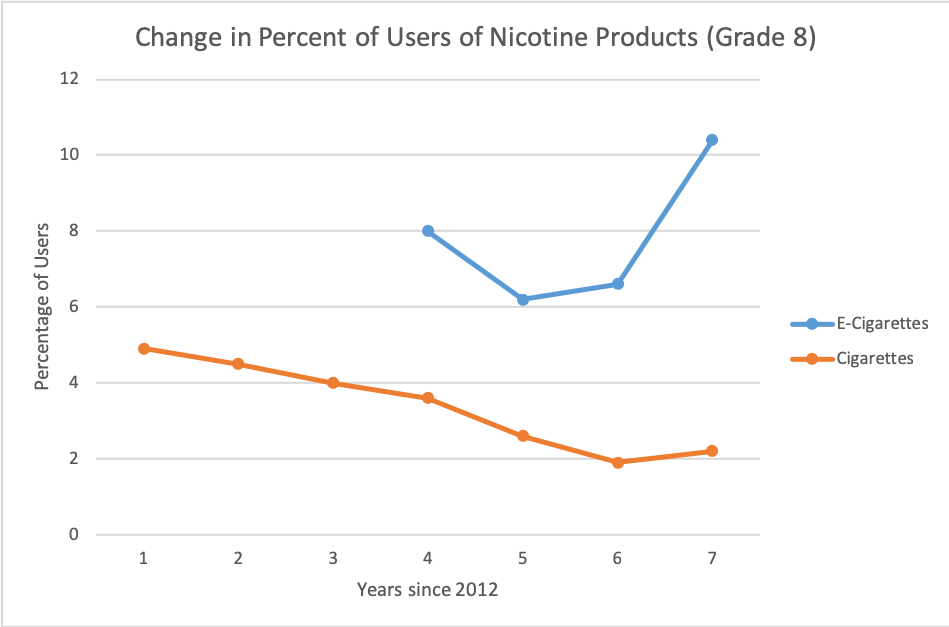
\includegraphics[width=\linewidth]{percentUsers8}
  \end{subfigure}
  \begin{subfigure}[t]{.3\linewidth}
  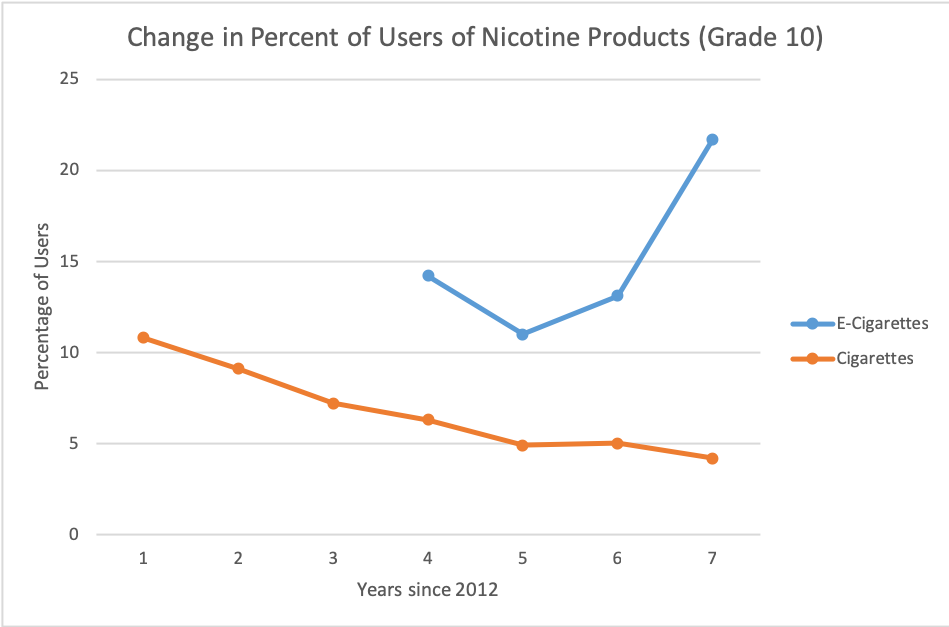
\includegraphics[width=\linewidth]{percentUsers10}
  \end{subfigure}
  \begin{subfigure}[t]{.3\linewidth}
  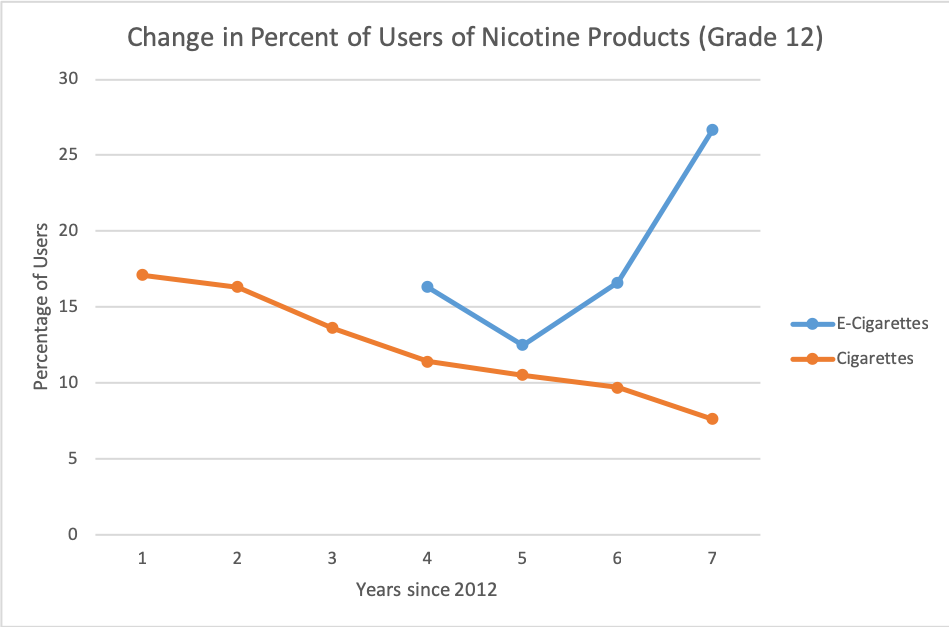
\includegraphics[width=\linewidth]{percentUsers12}
  \end{subfigure}
  
  \begin{subfigure}[t]{.4\linewidth}
  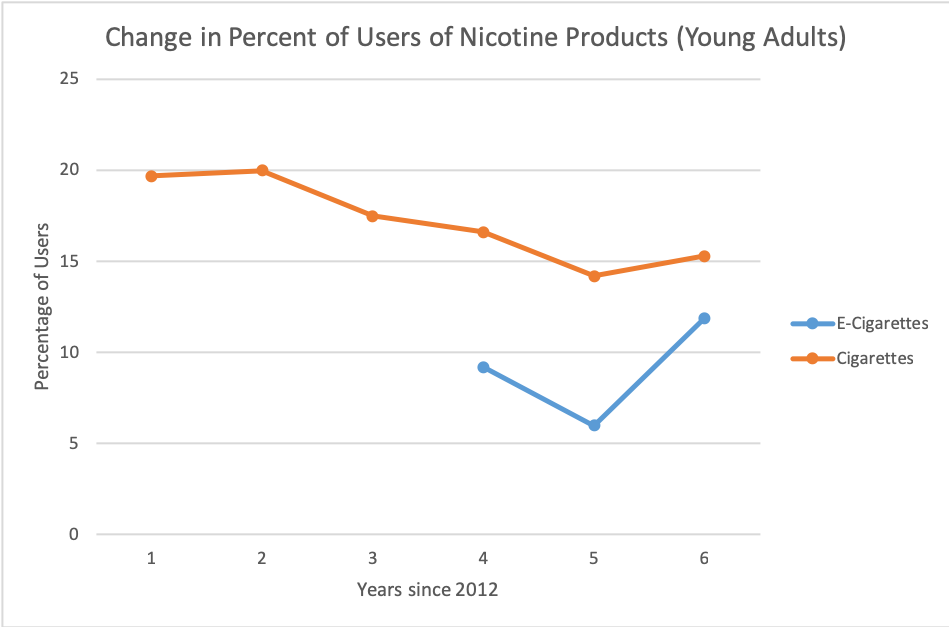
\includegraphics[width=\linewidth]{percentUsersYA}
  \end{subfigure}
  \begin{subfigure}[t]{.4\linewidth}
  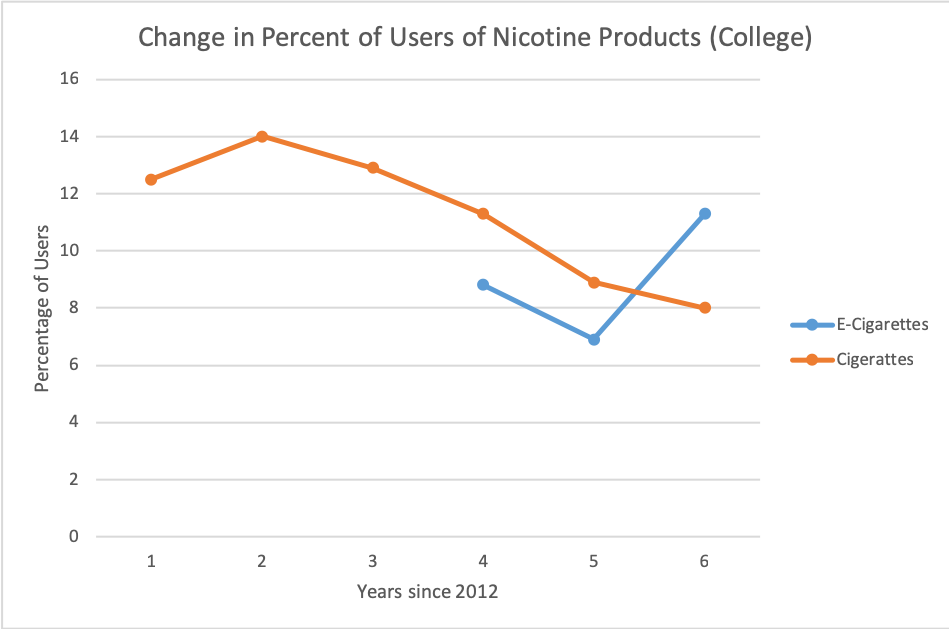
\includegraphics[width=\linewidth]{percentUsersCo}
  \end{subfigure}
  \caption{Vape vs. Cigarette Usage by Age Group \citep{noauthor_college-age_2018}}
\end{figure}

\subsection{Local Assumptions}
\begin{itemize}
  \item One cigarette contains 12 mg of nicotine \citep{matthews_how_2017}
  \item The rate of absorption of nicotine from one cigarette is 1 mg per cigarette because there is loss from the combustion of the cigarette and filtering. Our unit of 1 cigarette of nicotine indicates the rate of nicotine intake, 1 mg per cigarette, and not nicotine content, 12 mg per cigarette. \citep[501]{benowitz_daily_1984}
  \item One cigarette is worth 10 puffs. \citep{noauthor_e-cigarette_2014}
  \item One pack of cigarettes costs \$5 and contains 20 cigarettes.
  \item The current smoking rate among adults in the US is 14\%.
  \item Our model assumes JUULs as the unit of vape consumption and encapsulates e-cigarettes for this model.
  \item The JUUL device kit costs \$35 for the device and charger and is the base cost of entry for JUUL. \citep{noauthor_juul_nodate}
  \item Four JUUL pods cost \$16. \citep{noauthor_buy_nodate}
  \item A JUUL pod has negligible nicotine waste becasue there is no combustion or filter.
  \item One JUUL pod 41 mg or approximately 41 cigarettes worth of nicotine absorption. \citep{noauthor_juulpods_nodate}
  \item Our model only considers a death directly from overdose of nicotine, which is so unlikely that we have not accounted for it in our model.
\end{itemize}

\subsection{Cost Analysis of JUULs vs. Cigarettes}
To determine which nicotine vector is more cost effective over time, two linear equations were constructed for each, where $y$ is the total cost and $x$ is each additional cigarette (synonymous with each additional intake of 1 mg of nicotine).

\begin{figure}[H]
  \centering
  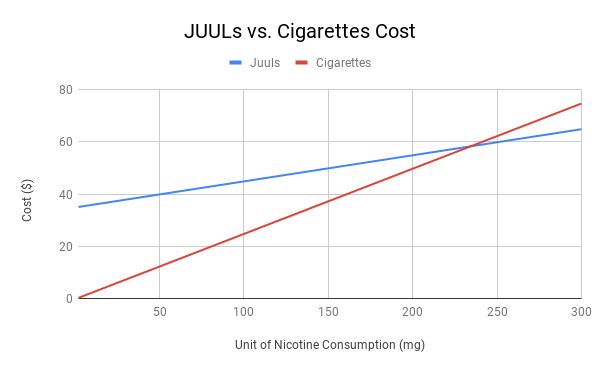
\includegraphics[width=.8\linewidth]{JUULs-vs-Cigarettes-Cost}
  \caption{JUULs vs. Cigarettes Cost}
  \label{fig:cigcosts}
  JUUL: $y = \frac{16}{160} x + 35$
  \begin{itemize}
  	\item Slope $\frac{16}{160}$ = cost per each additional cigarette, aka each additional cigarette worth of nicotine intake (1 mg).
  	  \subitem 16 = the cost of four JUUL pods; JUUL pods are sold in packs of four for \$15.99.
  	  \subitem 160 = the number of milligrams of nicotine in 4 pods (approximately 40 milligrams of nicotine per pod).
  	\item 35 = cost of device kit (\$34.99), which includes a JUUL device and charger.
  \end{itemize}
  Cigarette: $y = \frac{5}{20} x$
  \begin{itemize}
    \item Slope $\frac{5}{20}$ = Cost per each additional cigarette, aka each additional cigarette’s worth of nicotine intake (1 mg).
      \subitem 5 = simplified cost per pack of cigarette.
      \subitem 20 = number of milligrams of nicotine absorbed per pack.
  \end{itemize}
\end{figure}

\subsection{Model}

\begin{figure}[H]
  \centering
  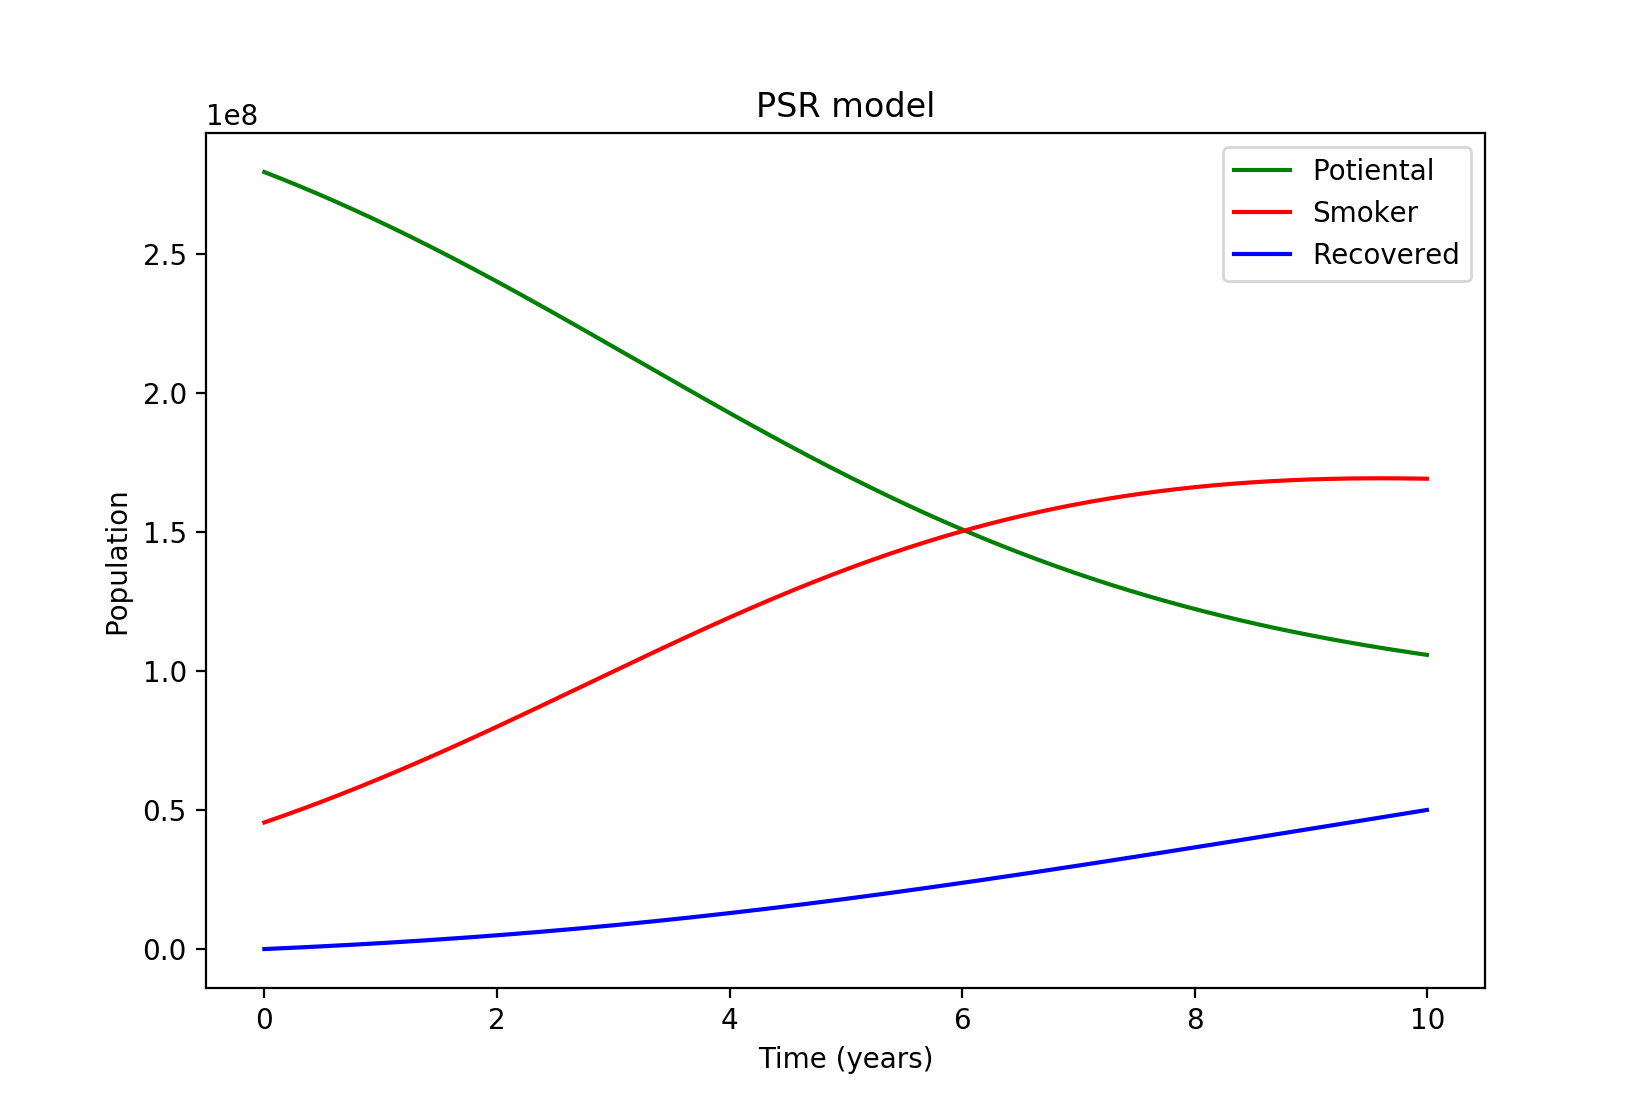
\includegraphics[width=.8\linewidth]{PSR}
  \caption{PSR for the total US population}
  \label{fig:PSR}
\end{figure}

\begin{singlespace}
\begin{small}
\begin{equation}
\label{eq:1}
\begin{aligned}
\frac{dP}{dt} &= \beta \frac{PS}{N} + \alpha ( 1 - \epsilon )S \\
\frac{dS}{dt} &= \beta \frac{PS}{N} - \alpha S \\
\frac{dQ}{dt} &= \alpha \epsilon S
\end{aligned}
\end{equation}
\begin{itemize}[label=]
  \item $S$ = Smokers
  \item $P$ = Potential smokers
  \item $\beta$ = Rate of transmission
  \item $\alpha$ = Rate of recovery
  \item $1 - \epsilon$ = Rate of relapse
  \item $Q$ = Smoking quitters
  \item $N$ = Total population
\end{itemize}
\end{small}
\end{singlespace}

\section{Above or Under the Influence?}

\subsection{Local Assumptions}

\begin{itemize}
  \item The proportion of deaths caused by opium overdose is negligible.
  \item The gateway nature of ateway nature of marijuana doesn’t need to be identified as its own variable because the reasons (behind why marijuana leads to opioid usage) can be woven into the other variables.
\end{itemize}

\subsection{Model}

\paragraph{Variables}
\begin{itemize}[label=]
  \item $S$ = Socioeconomic factors
  \item $P$ = People (social circles)
  \item $\beta$ = Baseline (derived from previous years)
  \item $N$ = Population
  \item $h$ = Health
  \item $x$ = Number of people
  \item $D$ = Death constant
\end{itemize}
\section{Ripples}

\subsection{Variables}

\begin{itemize}[label=]
  \item $C$ = Total cost of drug
  \item $T$ = Tax
  \item $c_j$ = Cost of jail
  \item $p_j$ = Percent of drug users in jail
  \item $p_r$ = Percent in rehab
  \item $c_r$ = Cost of rehab
  \item $M$ = Medical costs
\end{itemize}

\subsection{Local Assumptions}

\subsection{Conclusion}

\begin{enumerate}
  \item
\end{enumerate}


\newpage
\printbibliography
% \bibliographystyle{IEEEtran}
\newpage

\appendix
\listoffigures
\listoftables

\section{Listings}
\end{document}